% Fruit Ninja VR - Part 1 - Rapport (version courte)
% Compilation : pdflatex x2 (la version longue est conservée dans rapport-v1.tex)
\documentclass[11pt,a4paper]{article}

\usepackage[T1]{fontenc}
\usepackage[utf8]{inputenc}
\usepackage{lmodern}
\usepackage[french]{babel}
\usepackage[a4paper,margin=2.3cm]{geometry}
\usepackage{graphicx}
\usepackage{booktabs}
\usepackage{tabularx}
\usepackage{array}
\usepackage{enumitem}
\usepackage{caption}
\usepackage{float}
\usepackage{fancyhdr}
\usepackage[hidelinks]{hyperref}

\graphicspath{{../captures/}}
\setlist{nosep,leftmargin=*}
\captionsetup{font=small,labelfont=bf}
\setlength{\parskip}{0.5em}
\setlength{\parindent}{0pt}
\renewcommand{\arraystretch}{1.15}
\newcolumntype{L}{>{\raggedright\arraybackslash}X}
\newcolumntype{P}[1]{>{\raggedright\arraybackslash}p{#1}}
\newcommand{\fichier}[1]{\texttt{\small #1}}

\pagestyle{fancy}
\fancyhf{}
\lhead{\small Fruit Ninja VR -- Part 1}
\rhead{\small Junghoon KIM -- ST2VAAS 2026-2027}
\cfoot{\small \thepage}
\renewcommand{\headrulewidth}{0.4pt}

\begin{document}

\begin{center}
  {\LARGE\bfseries Fruit Ninja VR -- Part 1}\\[4pt]
  {\Large Reprise et déploiement multiplateforme}\\[10pt]
  ST2VAAS 2026-2027 \quad--\quad Junghoon KIM (groupe d'une personne)\\[4pt]
  Projet : \url{https://github.com/Ethervel/FruitNinjaVR}, branche \texttt{part1}, tag \texttt{part1-remise}\\[2pt]
  {\small Unity 6000.0.56f1 -- URP 17.0.4 -- OpenXR 1.15.1 -- XR Interaction Toolkit 3.0.8}
\end{center}

\vspace{0.5em}

% =====================================================================
\section{Le projet de départ et ce que j'ai remis en ordre}

J'ai repris mon mini-projet du S7, un Fruit Ninja en VR (dépôt \texttt{LaelKim/Fruit\_Ninja}, commit
\texttt{2db0f77} du 26/10/2025). Dans le dépôt de remise, cette version d'origine est sur la branche
\texttt{main} (tag \texttt{s7-initial}) ; tout le travail de la Part 1 est sur la branche \texttt{part1}.

J'ai d'abord installé la version exacte d'Unity du projet, 6000.0.56f1, pour ne pas le faire migrer
sans le vouloir. Ensuite j'ai lu le code et les scènes, et j'ai écrit un petit script d'audit
(\fichier{ProjectAudit.cs}) qui cherche les erreurs de compilation, les références cassées, les scripts
manquants et les matériaux non URP. Voici ce que j'ai trouvé.

\begin{table}[H]
\centering\small
\caption{État du projet S7 au départ.}
\begin{tabularx}{\textwidth}{@{}P{3.6cm}L@{}}
\toprule
Élément & Constat \\
\midrule
Rendu et XR & URP 17.0.4 ; OpenXR 1.15.1 et XR Interaction Toolkit 3.0.8 ; profil Oculus Touch sur PC \\
XR sur Android & \textbf{aucun loader}, Meta Quest Support désactivé : un APK aurait démarré sans VR \\
Entrées & Input System 1.14.2, mais \emph{Active Input Handling} réglé sur « Both » \\
Rig & ancien \texttt{XRRig} avec \texttt{TrackedPoseDriver} (legacy), pas d'XR Origin \\
Jeu & deux katanas, lancement de 8 fruits depuis 4 points, coupe du mesh, bombes, score et combo,
4 difficultés, partie de 120~s, menus : présents et cohérents \\
Absents du code & fruits bonus (champs déclarés mais jamais utilisés), réglage du volume, mode
entraînement, classement, sauvegarde JSON \\
Divers & deux fichiers C\# qui ne portaient pas le nom de leur classe ; un son de bombe joué en double ;
objets de test et \texttt{Debug.Log} laissés dans la scène \\
\bottomrule
\end{tabularx}
\end{table}

J'ai ajouté le fruit bonus, puisque le jeu le prévoyait déjà : une pomme dorée qui sort dans 7~\% des
tirs et rapporte 50 points. J'ai corrigé le son en double et renommé les deux scripts
(\fichier{FruitSpawner.cs}, \fichier{DestroyFloor.cs}). En revanche, je n'ai pas recréé le volume,
l'entraînement, le classement ni la sauvegarde JSON : ils n'existaient pas dans la version remise au
S7, et je les signale plutôt que de les inventer.

\paragraph{Organisation.} La racine d'\texttt{Assets} mélangeait tout. J'ai rangé le projet en dossiers
par rôle : \texttt{Scenes}, \texttt{Scripts} (par thème : \texttt{Core}, \texttt{Gameplay},
\texttt{Slicing}, \texttt{FX}\ldots), \texttt{Prefabs}, \texttt{Models}, \texttt{Materials},
\texttt{Textures}, \texttt{Audio}, \texttt{FX}, et un dossier \texttt{\_Unused} pour ce qui ne sert
plus. J'ai fait tous les déplacements avec l'API de l'éditeur (\texttt{AssetDatabase.MoveAsset}) et
jamais dans l'explorateur Windows : comme les \texttt{.meta} et les GUID suivent, aucune référence ne
casse. Après chaque étape, l'audit donnait 0 erreur, 0 référence cassée et 0 script manquant. Le jeu
tient dans une seule scène, \texttt{FruitNinjaVR\_Main} : accueil, choix de la difficulté, partie de
120~s, puis écran de fin avec Rejouer et Menu.

% =====================================================================
\section{Les effets de particules, en version PC et en version Quest}

J'ai fait deux effets. Le premier est une éclaboussure de jus au point où la lame touche le fruit,
de la couleur du fruit. Le second est une explosion de bombe : petite à chaque touche, au moment où
on perd des points, puis complète à la 3\textsuperscript{e} touche, avec le son et le flash qui
existaient déjà.

Chaque effet existe en deux variantes. Un composant, \texttt{GameFX}, choisit la bonne tout seul : la
variante Quest si le jeu est compilé pour Android, la variante PC sinon. Il écrit aussi son choix dans
le journal, ce qui m'a permis de vérifier ensuite que chaque build utilisait la bonne. Les prefabs sont
générés par un script éditeur, donc je peux les refaire à l'identique.

\paragraph{Pourquoi alléger sur le Quest.} Sur un GPU mobile, ce qui coûte le plus avec des
particules, c'est l'\emph{overdraw} : chaque particule transparente oblige à redessiner les mêmes
pixels plusieurs fois. J'ai donc d'abord réduit le nombre de particules. J'ai aussi retiré un
sous-système par effet, parce que chacun ajoute une simulation et un appel de dessin. Enfin, j'ai
enlevé ce qui coûte cher par particule : les collisions avec le décor, le bruit de turbulence,
l'éclairage par pixel et les \emph{soft particles}, qui ont besoin de la texture de profondeur. Pour
que l'effet reste lisible malgré tout, les gouttes du Quest sont moins nombreuses mais plus grosses.

\begin{table}[H]
\centering\small
\caption{Réglages principaux des deux effets.}
\begin{tabularx}{\textwidth}{@{}P{3.0cm}P{4.3cm}P{3.6cm}L@{}}
\toprule
 & PC & Quest & Pourquoi \\
\midrule
\multicolumn{4}{@{}l}{\textit{Éclaboussure de jus}} \\
Sous-systèmes & 2 (gouttes + brume) & 1 (gouttes) & une simulation de moins \\
Particules (burst / max) & 85 / 110 & 20 / 24 & overdraw \\
Gouttes & 0,015--0,04 m, étirées & 0,035--0,06 m, Billboard & moins, mais visibles \\
Collision, matériau & rebond sur le décor ; Lit, soft particles & aucune ; Unlit & coût par particule \\
\midrule
\multicolumn{4}{@{}l}{\textit{Explosion de bombe}} \\
Sous-systèmes & 4 (flash, feu, étincelles, fumée) & 3 (sans fumée) & la fumée crée le plus d'overdraw \\
Particules (burst / max) & 186 / 221 & 41 / 51 & divisé par 4,5 environ \\
Boule de feu & additive, avec bruit & alpha blend, sans bruit & voir ci-dessous \\
\bottomrule
\end{tabularx}
\end{table}

Pour la boule de feu, j'ai d'abord gardé le mode additif sur le Quest, mais sans HDR ni bloom elle
disparaissait presque sur le décor clair du dojo. Je suis passé en alpha blend avec des particules
plus grosses, et l'explosion se voit de nouveau. Les deux variantes partagent une seule petite texture
de 64$\times$64 pixels.

Pour comparer, j'ai rendu les deux variantes dans l'éditeur, depuis la hauteur des yeux du joueur
(1,6~m), avec le même cadrage et au même instant (0,12~s après la coupe pour le jus, 0,25~s pour la
bombe). Ce ne sont pas des captures du casque ; la teinte du décor change parce que le Quest utilise le
niveau de qualité \texttt{Mobile}, sans HDR ni post-process.

\begin{figure}[H]
\centering
\begin{tabular}{@{}cc@{}}
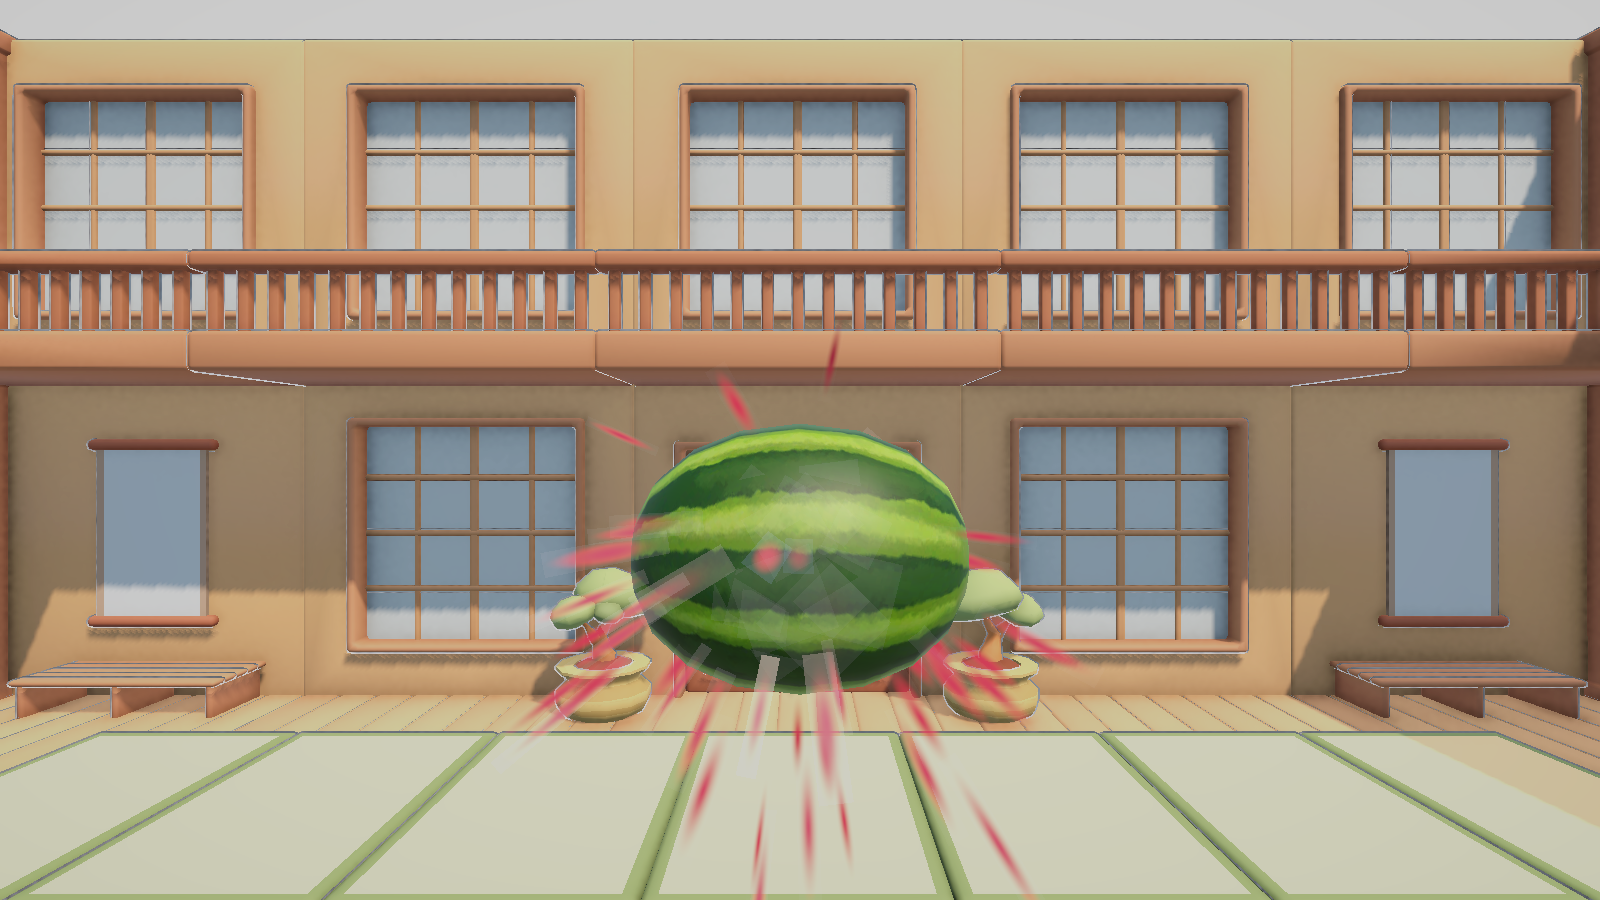
\includegraphics[width=0.46\textwidth]{FX_FruitJuice_PCVR.png} &
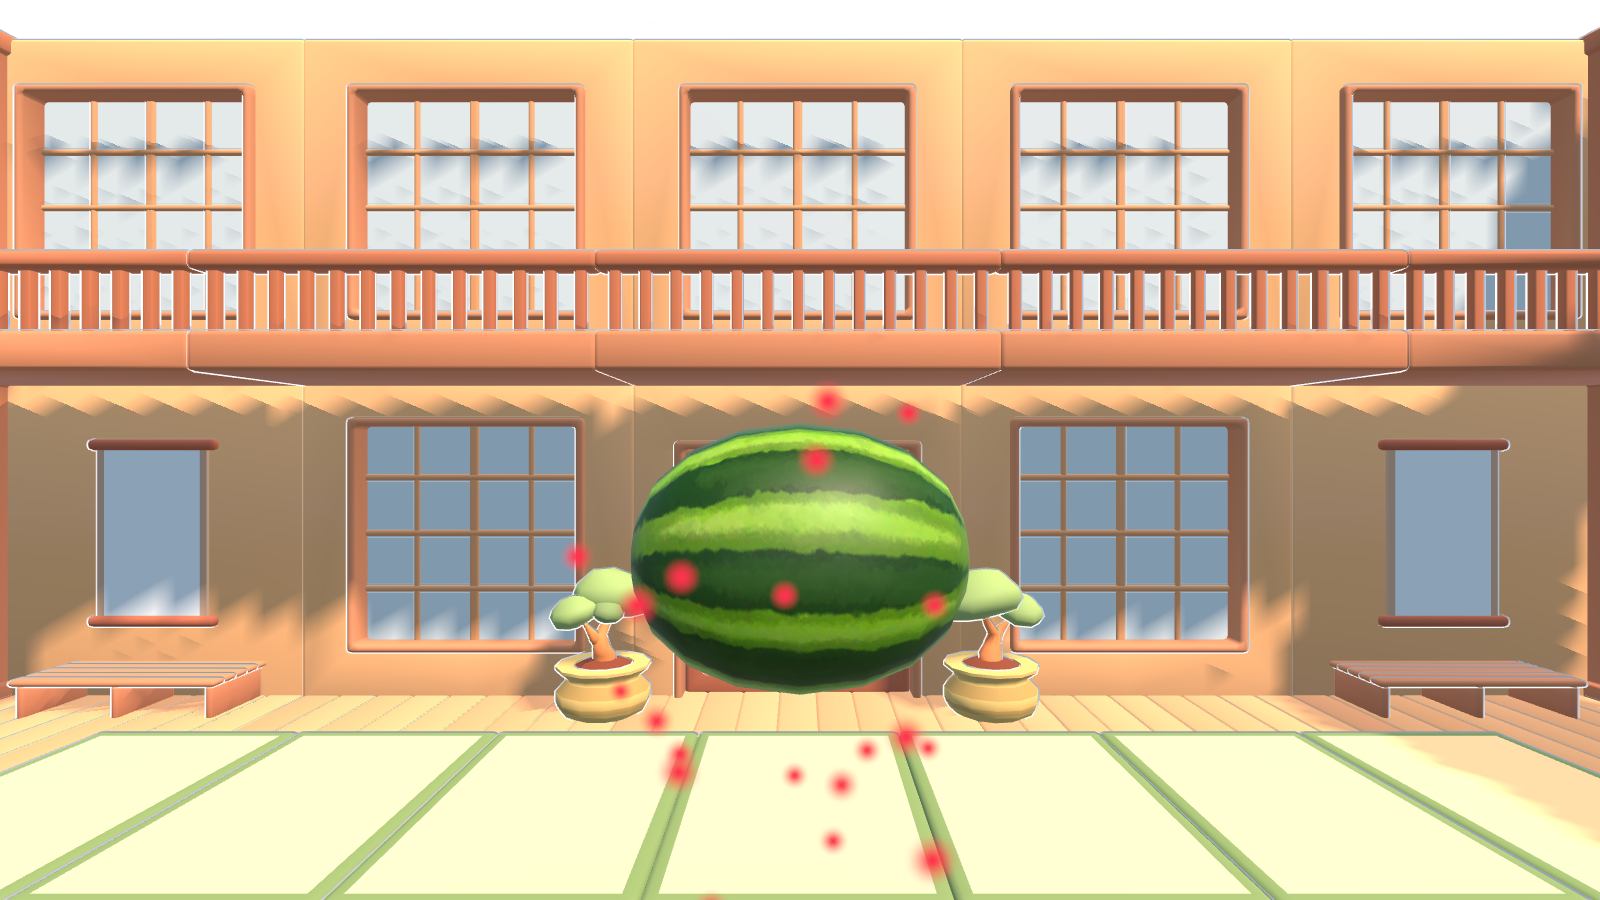
\includegraphics[width=0.46\textwidth]{FX_FruitJuice_Quest.png} \\
\small Jus -- PC (85 particules) & \small Jus -- Quest (20 particules) \\[4pt]
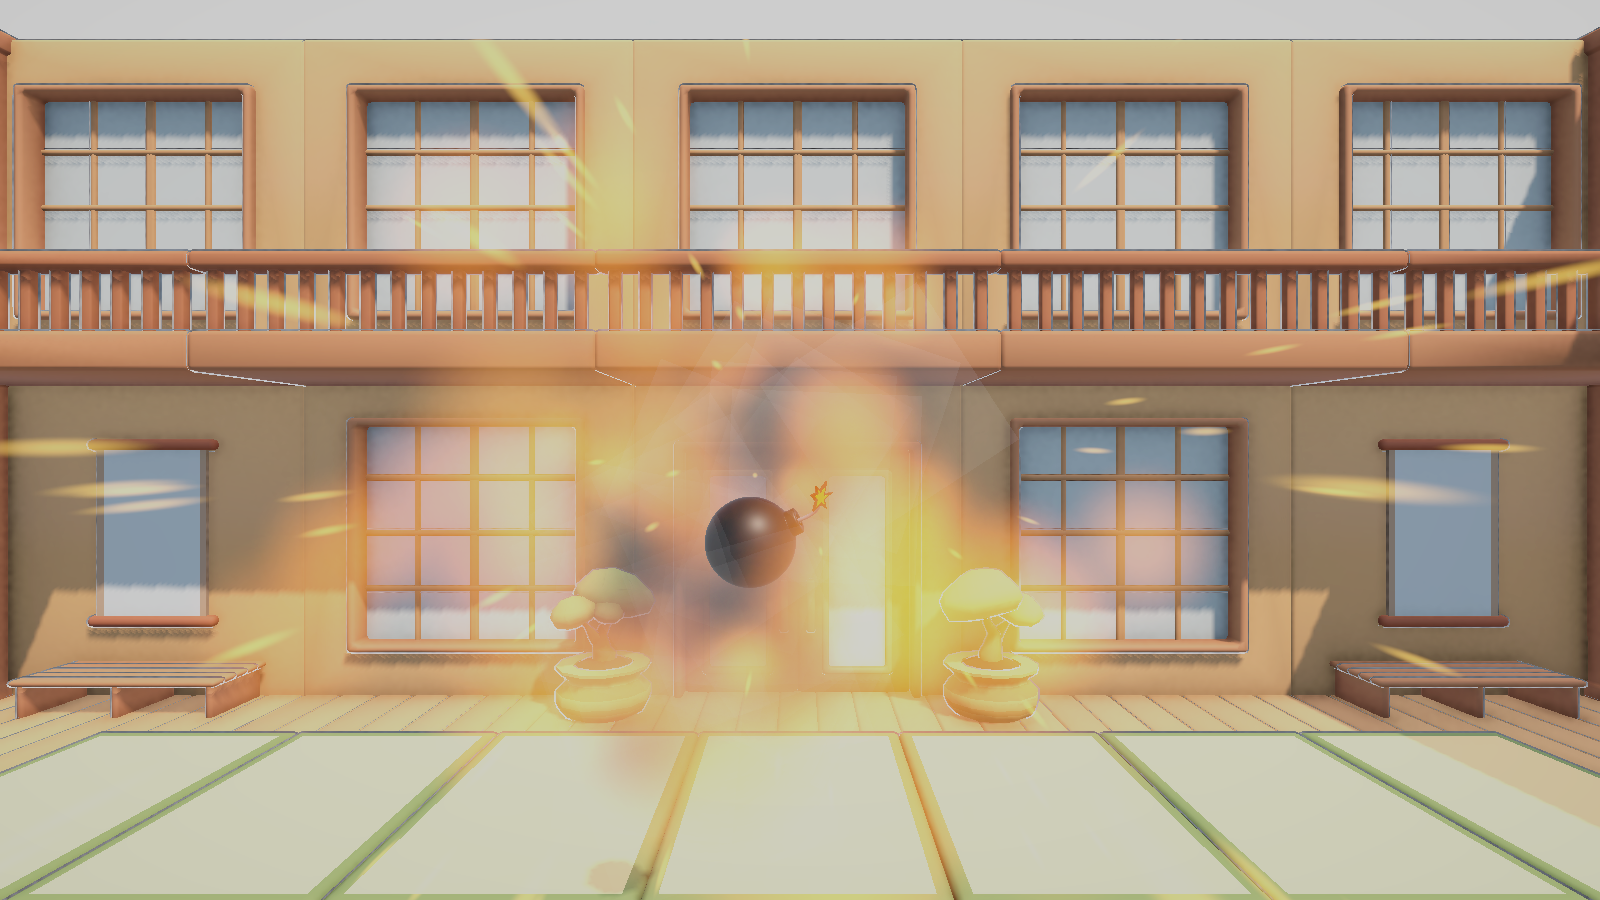
\includegraphics[width=0.46\textwidth]{FX_BombExplosion_PCVR.png} &
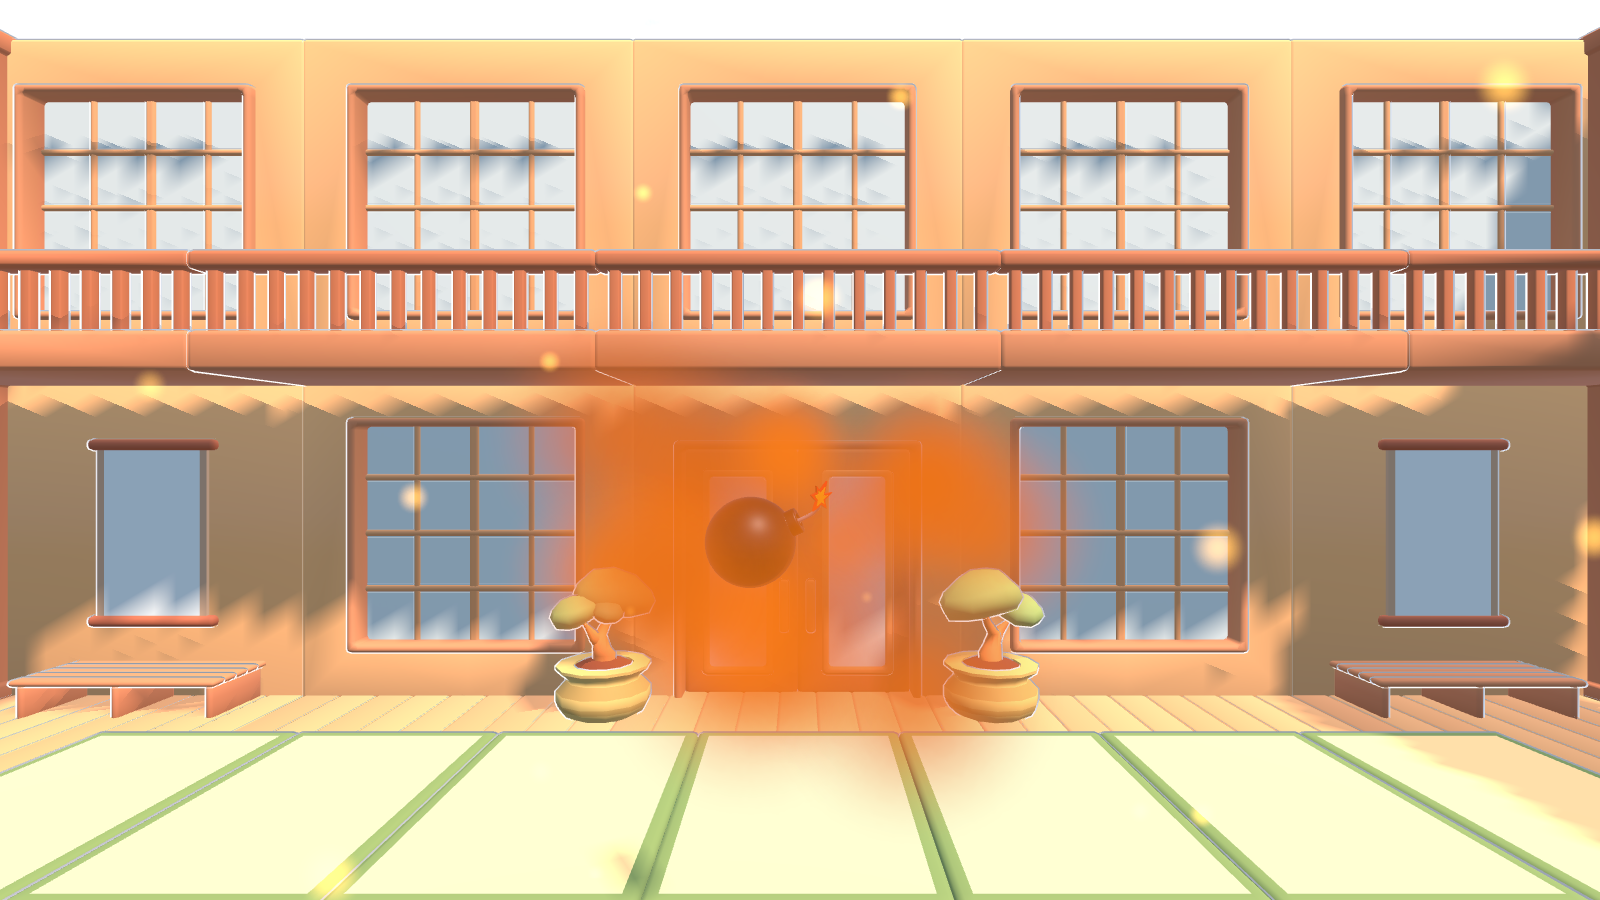
\includegraphics[width=0.46\textwidth]{FX_BombExplosion_Quest.png} \\
\small Explosion -- PC (185 particules) & \small Explosion -- Quest (40 particules) \\
\end{tabular}
\caption{Les deux effets rendus dans l'éditeur : PC à gauche, Quest à droite.}
\label{fig:fx}
\end{figure}

% =====================================================================
\section{Les builds et les tests au casque}

\paragraph{Réglages des builds.} J'ai écrit un script qui construit les deux versions et note les
réglages utilisés (menus \texttt{Tools > Fruit Ninja}). La version PC est en Mono, x86\_64, Direct3D~11,
textures BC, niveau de qualité \texttt{PC} (HDR, SSAO, ombres douces, post-process). La version Quest
est en IL2CPP, ARM64 uniquement, Vulkan, textures ASTC, niveau \texttt{Mobile} (MSAA 4x, sans HDR ni
post-process), API Android minimale 29 et cible automatique (36). Les deux utilisent OpenXR, le rendu
Single Pass Instanced, l'Input System seul et la seule scène \texttt{FruitNinjaVR\_Main}.

Je ne connaissais pas les réglages Android vus en cours. J'ai donc suivi les recommandations de Meta
et le profil Meta Quest d'Unity 6 ; il faudra les comparer à ceux du cours. Il a aussi fallu activer
OpenXR et Meta Quest Support pour Android, et passer l'Input System en mode seul, car le mode « Both »
n'est pas accepté sur Android. J'ai gardé le rig du S7 : il fonctionne sur les deux plateformes, car
OpenXR fournit les poses dont il a besoin. La validation OpenXR ne laisse qu'un avertissement sur le
SSAO pour Android ; c'est un faux positif, puisque le SSAO n'est que dans le rendu PC.

\paragraph{Matériel.} PC sous Windows 11 (i9-14900KF, RTX 3080, 32 Go). Casque Meta Quest 3 sous Meta
Horizon OS v205 (Android 14), écran à 72~Hz pendant le test. Pour le PC, Meta Horizon Link (runtime
1.208.0) par câble USB-C.

\paragraph{Comment j'ai testé.} Sur le Quest, j'ai fait deux sessions. Pendant la première, avec le
câble, la connexion adb tombait sans arrêt, parce que Link, ouvert sur le PC, utilisait le même câble.
J'ai donc refait le test sans câble : j'ai agrandi le journal du casque avant de jouer, puis je l'ai
relu en rebranchant. Les captures d'écran par adb sortaient noires ; j'ai pris les captures du casque
lui-même (bouton Meta + gâchette). Pour les FPS du Quest, j'ai lu les statistiques du compositeur Meta
dans le journal (une ligne par seconde). Pour le PC, j'ai activé le HUD de performance de Link et je
l'ai capturé toutes les 2~s dans la fenêtre Oculus Mirror.

La grille ci-dessous reprend le retour du joueur, qui a répondu « tout OK » sur les deux builds. C'est
du déclaratif ; je marque (j) ce que j'ai pu confirmer aussi dans les journaux.

\begin{table}[H]
\centering\small
\caption{Grille de test résumée (OK : retour du joueur ; (j) : confirmé aussi par le journal).}
\begin{tabularx}{\textwidth}{@{}P{3.4cm}LP{2.0cm}P{2.0cm}@{}}
\toprule
Point & Ce qu'on vérifie & PC (Link) & Quest \\
\midrule
Démarrage & pas d'écran noir ni de crash & OK (j) & OK (j) \\
Tracking, katanas & tête, deux manettes, un katana par main & OK & OK \\
Menu & rayon et gâchette droite & OK & OK \\
Coupe, jus, combo & coupe nette, +10, jus coloré, combo +50, pomme dorée vue & OK (j) & OK (j) \\
Bombe touchée & $-25$ points, $-1$ vie, petite explosion & OK (j) & OK (j) \\
Explosion à 3 touches & tremblement, grande explosion, flash & non confirmée & non confirmée \\
Fin de partie, difficultés & écran de fin, vies selon le niveau & OK (j) & OK (j) \\
Lisibilité, fluidité & textes lisibles, pas de saccade & OK & OK \\
Stabilité & 2 parties sans crash & OK (j) & OK \\
Autonomie & jeu lancé sans câble ni PC & -- & OK (j) \\
\bottomrule
\end{tabularx}
\end{table}

Le journal confirme aussi la bonne variante d'effets sur chaque build (\texttt{[GameFX] variante
utilisée : Quest} et \texttt{: PCVR}), sans exception ni crash. L'explosion à 3 touches, elle, n'apparaît
dans aucun journal conservé : on n'y voit jamais plus de deux touches sur la même bombe. Le parcours que
j'avais prévu la testait en Extrême, où l'on n'a qu'une vie, donc la partie s'arrête à
la première touche. Il faudrait la tester en Facile (5 vies).

\begin{figure}[H]
\centering
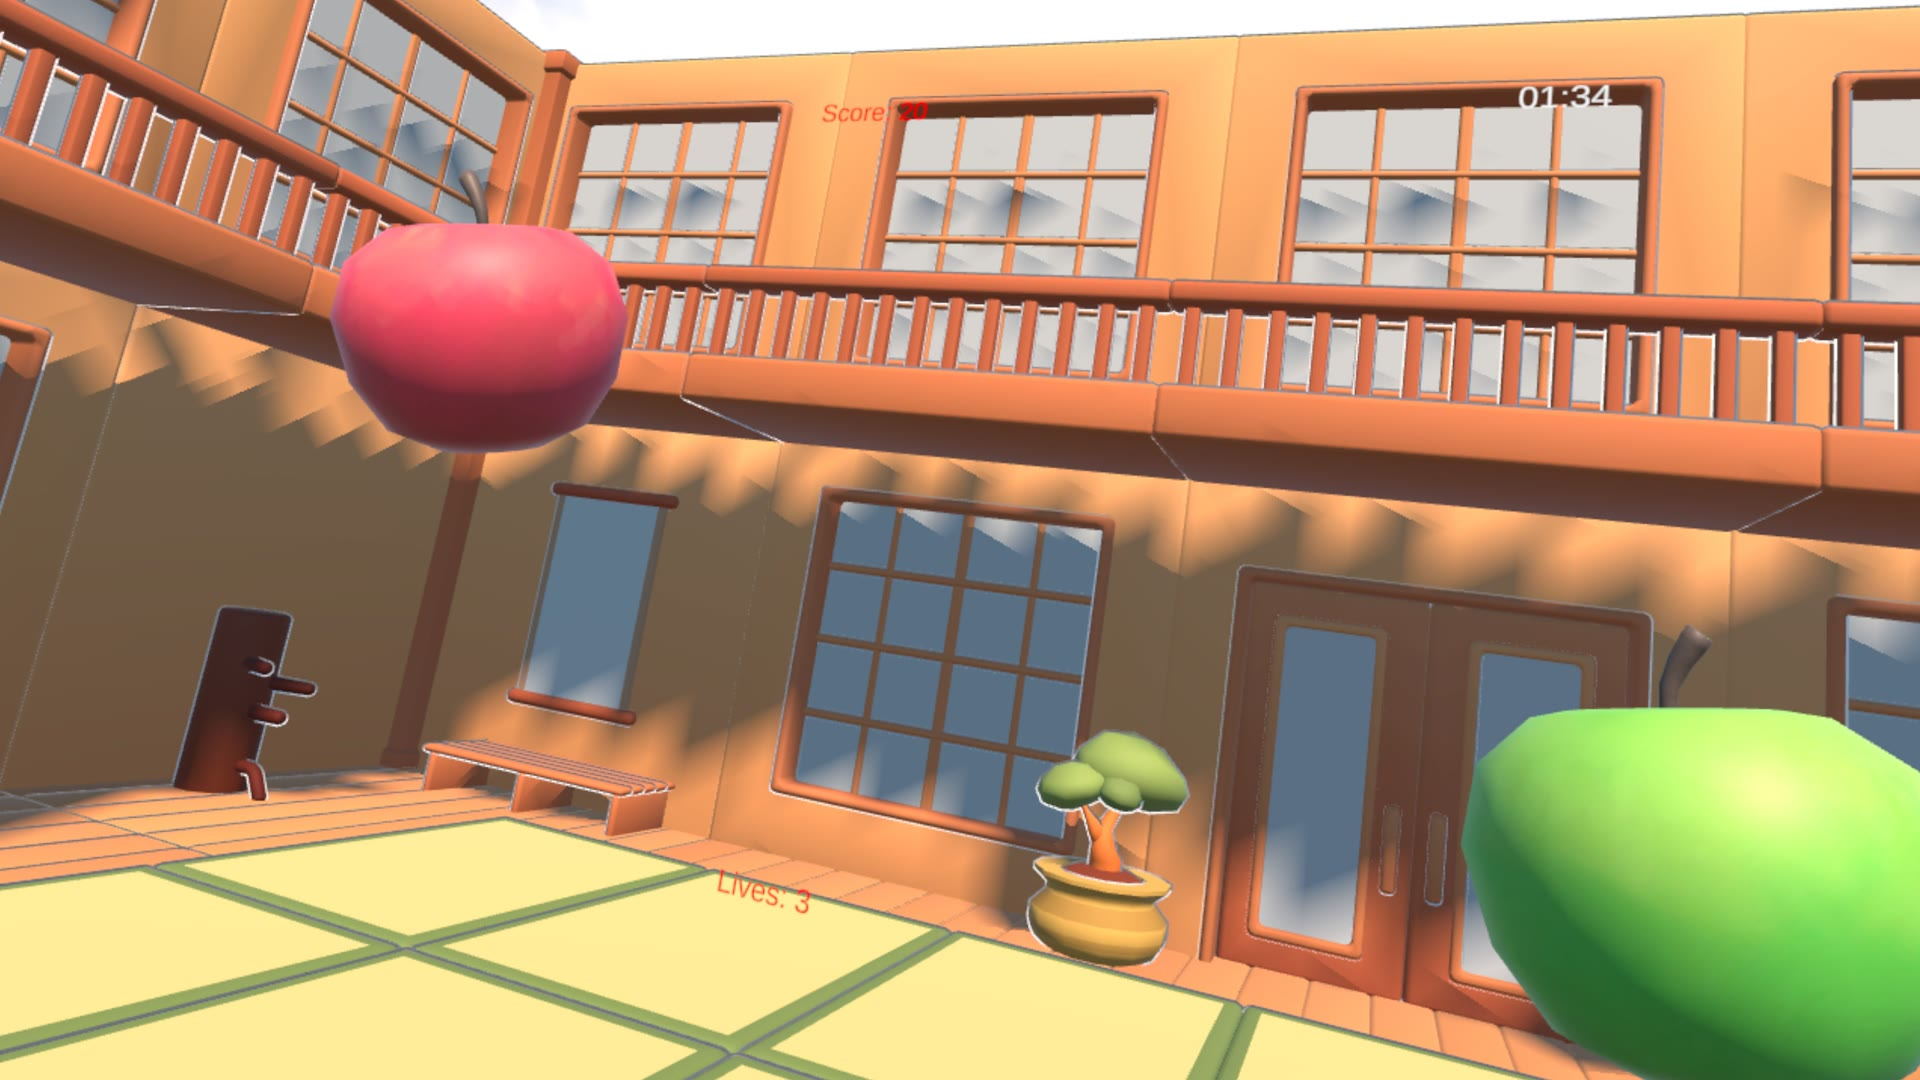
\includegraphics[width=0.7\textwidth]{quest/quest_jeu_fruits.jpg}
\caption{Capture prise dans le Quest 3 pendant une partie (vue d'un œil) : fruits en vol, score,
minuteur et vies.}
\label{fig:quest}
\end{figure}

\paragraph{Un bug trouvé grâce aux tests.} Les deux journaux répétaient l'erreur \texttt{Tag: Slice is
not defined} (42 fois sur le Quest, 122 sur le PC). Elle venait du script \texttt{DestroyFloor} du S7,
qui testait les morceaux tombés au sol avec un tag qui n'existe pas. Rien ne se voyait en jeu, mais
j'ai corrigé la ligne et refait les deux builds. Les tests au casque ont donc été faits avant ce
correctif : le nouvel APK est installé, mais je ne l'ai pas relancé au casque ; son build s'est terminé
sans erreur.

% =====================================================================
\section{L'APK, les tailles et la fluidité}

\paragraph{Les tailles.} J'ai ouvert l'APK dans l'APK Analyzer d'Android Studio. Il affiche
« APK size : 52.4 MB » et « Download Size : 47.4 MB ». Attention aux unités : ces « MB » sont en
fait des Mio (1~Mio = $2^{20}$ octets), alors que mon tableau est en Mo ($10^6$ octets). 52,4~Mio font
bien 54,98~Mo. La taille de téléchargement est une
estimation de l'outil pour une distribution par un store.

\begin{table}[H]
\centering\small
\caption{Tailles des builds finaux (1 Mo = $10^6$ octets).}
\begin{tabularx}{\textwidth}{@{}Lrr@{}}
\toprule
Fichier & Octets & Mo \\
\midrule
APK Quest & 54\,977\,835 & 54,98 \\
APK, taille de téléchargement estimée & 49\,709\,272 & 49,71 \\
Contenu de l'APK une fois décompressé & 149\,394\,197 & 149,39 \\
ZIP du build Windows & 71\,426\,270 & 71,43 \\
Dossier Windows livré & 152\,105\,649 & 152,11 \\
\bottomrule
\end{tabularx}
\end{table}

Il faut comparer ce qui est comparable. Un APK est déjà une archive ZIP : je le compare donc au ZIP
Windows, et son contenu décompressé au dossier Windows. L'APK réduit ses données à 36,8~\% de leur
taille, le ZIP Windows seulement à 47,0~\%. Les textures PC sont déjà très denses et le build Windows
contient en plus le moteur (\texttt{UnityPlayer.dll}) et les assemblies .NET.

Les captures de l'APK Analyzer viennent d'un build de la veille. Depuis, l'APK n'a changé que de
224 octets, ce qui ne change rien aux valeurs arrondies. Le dossier Windows, lui, a perdu 0,73~Mo :
j'utilisais pendant le développement un outil de pilotage de l'éditeur (MCP for Unity), et une petite
partie de cet outil se retrouvait dans le build PC. Je l'ai retiré avant la remise.

\begin{figure}[H]
\centering
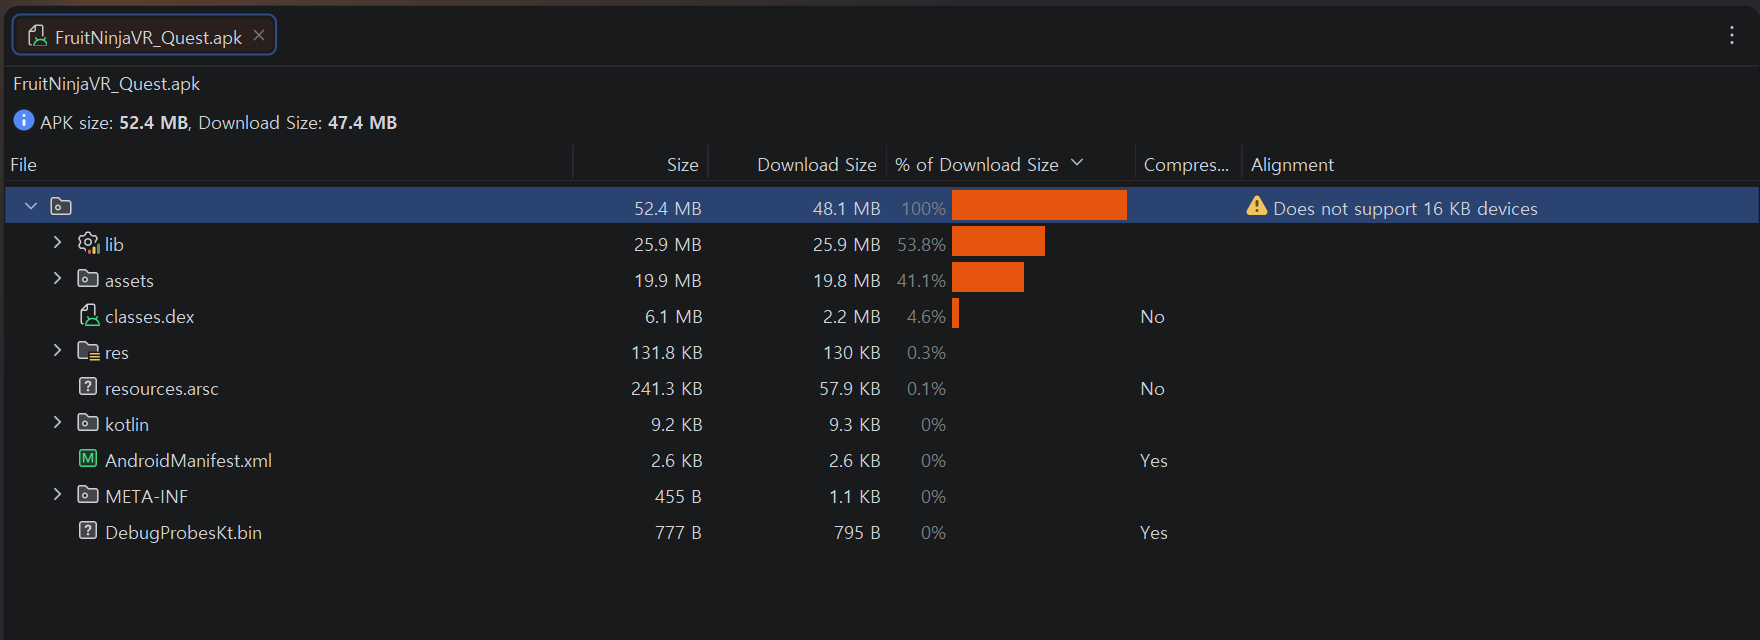
\includegraphics[width=0.88\textwidth]{apk-analyzer/01-vue-ensemble.png}
\caption{APK Analyzer : le code natif (\texttt{lib}) fait 53,8~\% du téléchargement, les données Unity
(\texttt{assets}) 41,1~\%.}
\label{fig:apk}
\end{figure}

\paragraph{Ce qui prend de la place.} Le plus gros poste est le code natif, environ la moitié de l'APK.
Le fichier \fichier{libil2cpp.so} pèse 16,2~Mo compressé (64,8~Mo décompressé). Il ne contient pas seulement la quinzaine de scripts du jeu : il contient tout le C\# des
paquets (XR Interaction Toolkit, Input System, URP\ldots), traduit en C++ par IL2CPP. Le
\emph{stripping} est réglé sur « Minimal » ; un réglage plus fort réduirait ce fichier, mais risquerait
de retirer du code que les paquets appellent par réflexion. Vient ensuite le moteur
(\fichier{libunity.so}, 9,5~Mo). Côté données, les textures font 73,5~\% des assets du jeu sur Android.
Le plus gros est le ciel HDR en 4K : 14,3~Mo en ASTC sur le Quest, contre 32,0~Mo en BC6H sur PC. Les
meshes, les shaders et les sons pèsent peu. L'outil affiche aussi « Does not support 16 KB devices » :
cela vient des deux bibliothèques OpenXR fournies par les paquets, que je ne peux pas modifier dans le
projet. Je n'ai constaté aucun effet sur le Quest 3, mais c'est un point à surveiller.

\paragraph{La fluidité.} Les deux builds tiennent les 72 images par seconde de l'écran. La différence
se voit dans la marge qui reste.

\begin{table}[H]
\centering\small
\caption{FPS mesurés en jeu (écran à 72~Hz).}
\begin{tabularx}{\textwidth}{@{}P{2.5cm}P{1.6cm}P{1.7cm}L@{}}
\toprule
Build, partie & Moyenne & Minimum & Remarques \\
\midrule
Quest, Normal & 72,5 & 71 & 85~s, aucune seconde sous 70 ; GPU occupé à 81~\% (88~\% au plus), CPU à 23~\% \\
Quest, Extrême & -- & -- & non mesuré (journal de la 1\textsuperscript{re} session perdu) \\
PC, Normal & 72,0 & 72 & 38~s mesurées, 1 image perdue ; marge de 77 à 84~\% \\
PC, Extrême & 72,0 & 72 & environ 40~s, aucune image perdue ; marge de 71 à 85~\% \\
\bottomrule
\end{tabularx}
\end{table}

Sur le Quest, la valeur 72,5 au-dessus de 72 vient de la façon dont le compteur découpe les secondes.
Le GPU met 9,4~ms par image en moyenne (10,0~ms au plus), pour un budget de 13,9~ms à 72~Hz : il reste
environ 28~\% de marge, et c'est bien le GPU qui limite, pas le CPU. Cela confirme qu'il fallait
alléger les particules. La seule baisse vient du chargement : une seconde à 64~FPS juste avant le menu.
Sur le PC, la RTX 3080 garde 71 à 85~\% de marge ; le seul creux, à 63~Hz, a lieu au retour au menu,
hors partie. Le PC pourrait donc afficher les effets complets sans problème, alors que le Quest a
besoin de sa version allégée.

À l'œil, les deux versions montrent le même décor et la même interface. Le PC a en plus l'éclairage
HDR, le post-process et des jus plus fournis. Le Quest est plus plat, mais les effets restent lisibles
et le joueur n'a signalé ni saccade ni texte illisible. Via Link, la latence mouvement-photon est
d'environ 43~ms ; c'est propre au streaming et n'existe pas en autonome.

% =====================================================================
\section{Difficultés, limites et bilan}

\paragraph{Ce qui m'a bloqué.} Le build Android échouait avec « Failed to update Android SDK ». La cause : \fichier{C:\textbackslash Windows\textbackslash System32} manquait
dans le PATH du poste : l'outil du SDK ne trouvait pas la commande \texttt{findstr}. J'ai lancé Unity
avec un PATH corrigé ; le PATH du poste reste à réparer. Le SDK 32 demandé par le projet n'était pas
installé, et le SDK d'Unity, sous \fichier{Program Files}, n'est pas modifiable sans droits
administrateur : j'ai mis la cible Android sur « Automatic », soit l'API 36. Pendant les tests, il y a
eu la connexion adb qui tombait à cause de Link, le journal du casque trop petit (256~Kio, écrasé en
quelques minutes) et les captures adb noires ; je les ai contournés comme décrit plus haut.

\paragraph{Limites que je laisse.}
\begin{itemize}
\item La grande explosion à 3 touches n'est pas confirmée par les journaux, et les FPS du Quest en
  Extrême n'ont pas été mesurés.
\item Le dernier APK, avec le correctif de \texttt{DestroyFloor}, est installé mais n'a pas été relancé
  au casque.
\item Le bouton Quitter du menu réagit au contact des katanas : pendant le test PC, le jeu s'est fermé
  après un retour au menu.
\item Volume, mode entraînement, classement et sauvegarde JSON restent absents, comme dans la version S7.
\item Le rig legacy du S7 est conservé, les réglages Android sont à confronter à ceux du cours, et il
  reste des objets de test et des \texttt{Debug.Log} dans la scène.
\item Le ciel HDR en 4K est le premier poste à réduire si la taille de l'APK ou la mémoire posent problème.
\end{itemize}

\paragraph{Conclusion : ce que j'en retiens.} D'abord, qu'il faut mesurer sur le casque plutôt que
deviner. Le Quest tient 72~FPS, mais avec une marge d'environ
28~\% seulement, et c'est le GPU qui limite. Sans les effets allégés, cette marge
aurait fondu. J'ai aussi compris pourquoi il faut déplacer les assets depuis l'éditeur et pas depuis
l'explorateur, et pourquoi une taille d'APK se lit avec ses unités et en comparant des archives entre
elles. Enfin, les journaux m'ont été très utiles : c'est grâce à eux que j'ai trouvé le bug du tag
\texttt{Slice}, qui ne se voyait pas en jeu.

\paragraph{Ce que je ferais autrement.} Je préparerais les mesures avant de jouer : journal du casque
agrandi dès le début, HUD de Link prêt, et un parcours de test pensé pour chaque point (l'explosion à
3 touches en Facile, pas en Extrême). Je ferais aussi tous les tests sur le build final, pour ne pas
avoir un correctif non revérifié au casque. Enfin, je retirerais plus tôt les outils de développement
du projet, puisque l'un d'eux s'était glissé dans le build PC.

\end{document}
